62. $f(x)=(x+1)|x-1|=\begin{cases} x^2-1,\ x\geqslant1,\\ 1-x^2,\ x<1.\end{cases}$
$$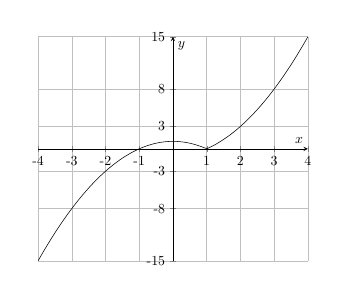
\begin{tikzpicture}[scale=0.5]
\begin{axis}[
    axis lines = middle,
    grid=major,
    legend pos={south west},
    xlabel = {$x$},
    %xlabel style={below right},
    ylabel = {$y$},
    ymin=-15,
    ymax=15,
    xmin=-4,
    xmax=4,
    xtick={-4,-2,-3,-1,1,2,3,4,6},
    xticklabels={-4,-2,-3,-1,1,2,3,4,6},
    ytick={-15,-3,-8,3,8,15},
    yticklabels={-15,-3,-8,3,8,15},
                  ]
	\addplot[domain=-4:4, samples=100, color=black] {(x+1)*abs(x-1)};
    %\addplot[domain=2.01:6, samples=100, color=black] {2/(2-x)};
   % \addplot[domain=-3:3, samples=100, color=black] {-x};
     %\addlegendentry{$\text{Рис. 1}$};
\end{axis}
%\draw (3.04,3.42) circle (2pt);
\end{tikzpicture}$$
По графику определим промежутки возрастания: $(-\infty;0]$ и $[1;+\infty).$\\
